\documentclass[11pt, a4paper]{article}
\usepackage{pdfpages}
\usepackage{parallel}
\usepackage[T2A]{fontenc}
\usepackage{ucs}
\usepackage[utf8x]{inputenc}
\usepackage[polish,english,russian]{babel}
\usepackage{hyperref}
\usepackage{rotating}
\usepackage[inner=2cm,top=1.8cm,outer=2cm,bottom=2.3cm,nohead]{geometry}
\usepackage{listings}
\usepackage{graphicx}
\usepackage{wrapfig}
\usepackage{longtable}
\usepackage{indentfirst}
\usepackage{array}
\usepackage{tikzsymbols}
\usepackage{soul}
\usepackage[ruled,vlined]{algorithm2e}
%\counterwithout{figure}{section} 

\usepackage{url}
\makeatletter
\g@addto@macro{\UrlBreaks}{\UrlOrds}
\makeatother

\newcolumntype{P}[1]{>{\raggedright\arraybackslash}p{#1}}
\frenchspacing
\usepackage{fixltx2e} %text sub- and superscripts
\usepackage{icomma} % коскі ў матэматычным рэжыме
\PreloadUnicodePage{4}

\newcommand{\longpage}{\enlargethispage{\baselineskip}}
\newcommand{\shortpage}{\enlargethispage{-\baselineskip}}

\def\switchlang#1{\expandafter\csname switchlang#1\endcsname}
\def\switchlangbe{
\let\saverefname=\refname%
\def\refname{Літаратура}%
\def\figurename{Іл.}%
}
\def\switchlangen{
\let\saverefname=\refname%
\def\refname{References}%
\def\figurename{Fig.}%
}
\def\switchlangru{
\let\saverefname=\refname%
\let\savefigurename=\figurename%
\def\refname{Литература}%
\def\figurename{Рис.}%
}

\hyphenation{admi-ni-stra-tive}
\hyphenation{ex-pe-ri-ence}
\hyphenation{fle-xi-bi-li-ty}
\hyphenation{Py-thon}
\hyphenation{ma-the-ma-ti-cal}
\hyphenation{re-ported}
\hyphenation{imp-le-menta-tions}
\hyphenation{pro-vides}
\hyphenation{en-gi-neering}
\hyphenation{com-pa-ti-bi-li-ty}
\hyphenation{im-pos-sible}
\hyphenation{desk-top}
\hyphenation{elec-tro-nic}
\hyphenation{com-pa-ny}
\hyphenation{de-ve-lop-ment}
\hyphenation{de-ve-loping}
\hyphenation{de-ve-lop}
\hyphenation{da-ta-ba-se}
\hyphenation{plat-forms}
\hyphenation{or-ga-ni-za-tion}
\hyphenation{pro-gramming}
\hyphenation{in-stru-ments}
\hyphenation{Li-nux}
\hyphenation{sour-ce}
\hyphenation{en-vi-ron-ment}
\hyphenation{Te-le-pathy}
\hyphenation{Li-nux-ov-ka}
\hyphenation{Open-BSD}
\hyphenation{Free-BSD}
\hyphenation{men-ti-on-ed}
\hyphenation{app-li-ca-tion}

\def\progref!#1!{\texttt{#1}}
\renewcommand{\arraystretch}{2} %Іначай формулы ў матрыцы зліпаюцца з лініямі
\usepackage{array}

\def\interview #1 (#2), #3, #4, #5\par{

\section[#1, #3, #4]{#1 -- #3, #4}
\def\qname{LVEE}
\def\aname{#1}
\def\q ##1\par{{\noindent \bf \qname: ##1 }\par}
\def\a{{\noindent \bf \aname: } \def\qname{L}\def\aname{#2}}
}

\def\interview* #1 (#2), #3, #4, #5\par{

\section*{#1\\{\small\rm #3, #4. #5}}
\ifx\ParallelWhichBox\undefined%
    \addcontentsline{toc}{section}{#1, #3, #4}%
\else%
\ifnum\ParallelWhichBox=0%
    \addcontentsline{toc}{section}{#1, #3, #4}%
\fi\fi%

\def\qname{LVEE}
\def\aname{#1}
\def\q ##1\par{{\noindent \bf \qname: ##1 }\par}
\def\a{{\noindent \bf \aname: } \def\qname{L}\def\aname{#2}}
}

\newcommand{\interviewfooter}[1]{
\vskip 1em
\noindent \textit{#1}
}

\switchlang{ru}
\begin{document}

\title{1983 "--- DEC VS10X-EA Mouse}
\date{}
\maketitle
\selectlanguage{russian}
Мышь DEC VS10X-EA (рис. \ref{fig:DecVS10XPic}) была выпущена в 1983 году на базе разработки компании Hawley Mouse House \cite{hawley,mouses}, созданной Джеком Хоули, соразработчиком мыши для компьютеров Xerox Alto и одним из авторов патента Xerox 1973 года на мышь с двумя наклонными колесами \cite{pat}. Фактически, DEC VS10X-EA является модификацией мыши Hawley Mark II X063X Mouse того же года выпуска. Сравнение двух мышей не выявляет конструктивных различий; все расхождения касаются формы корпуса и разъёма. Данной мышью комплектовались графические терминалы DEC VAXstation 100 \cite{reddit}, использовавшиеся при создании графической оконной системы Unix-подобных ОС, X Windows System.

\begin{figure}[h]
   \centering
    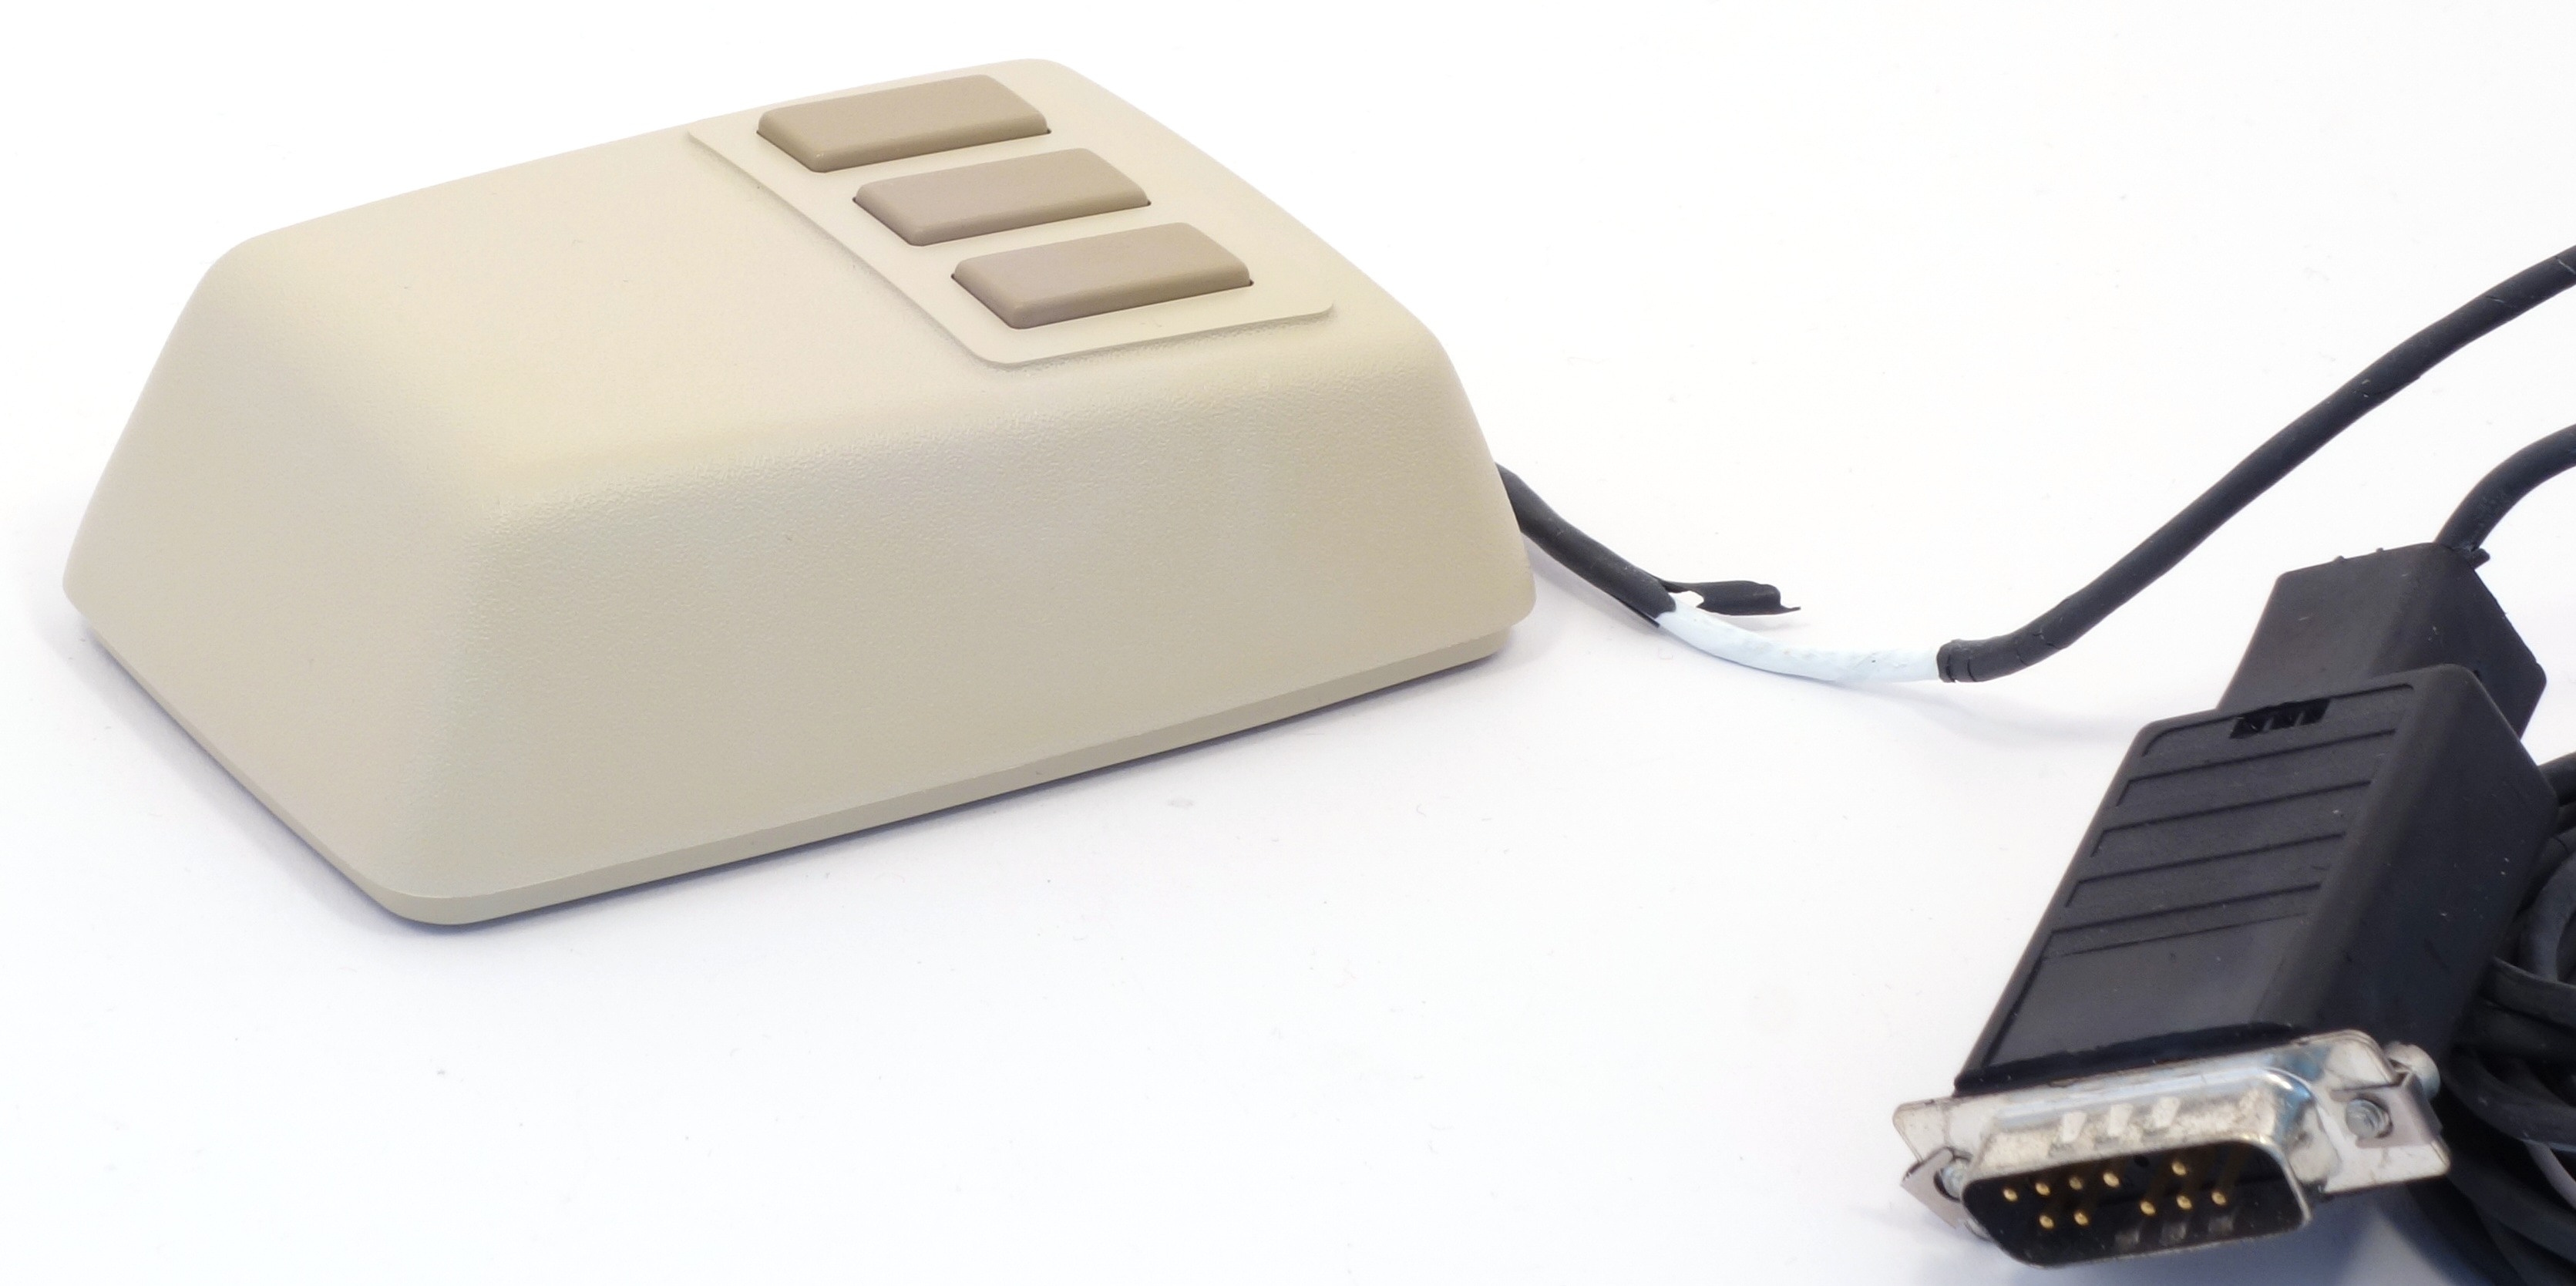
\includegraphics[scale=0.6]{1983_dec_vs10x_ea_mouse/pic_30.jpg}
    \caption{DEC VS10X-EA Mouse, вид спереди}
    \label{fig:DecVS10XPic}
\end{figure}

Если корпус мыши-прототипа, Hawley Mark II, представляет собой паралеллепипед, с тремя прямоугольные кнопки, то корпус DEC VS10X-EA имеет более сглаженную форму с большим наклоном стенок корпуса и плавными переходами между гранями. Достигается это за счет увеличенного корпуса, в который <<вписан>> легко узнаваемый прямоугольник мыши Hawley (рис. \ref{fig:DecVS10XTopAndBottom}). Очевидно, такой дизайн не мог не сказаться положительно на эргономике манипулятора.

\begin{figure}[h]
    \centering
    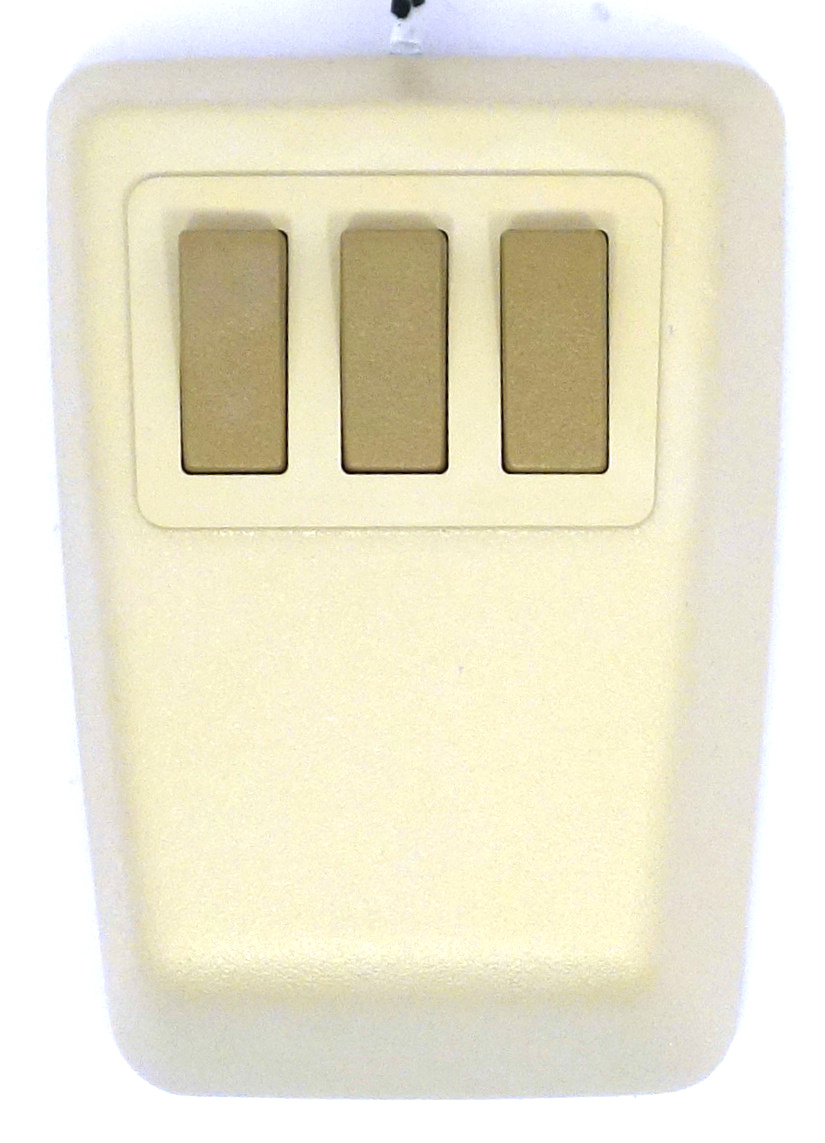
\includegraphics[scale=0.5]{1983_dec_vs10x_ea_mouse/top_60.jpg}
    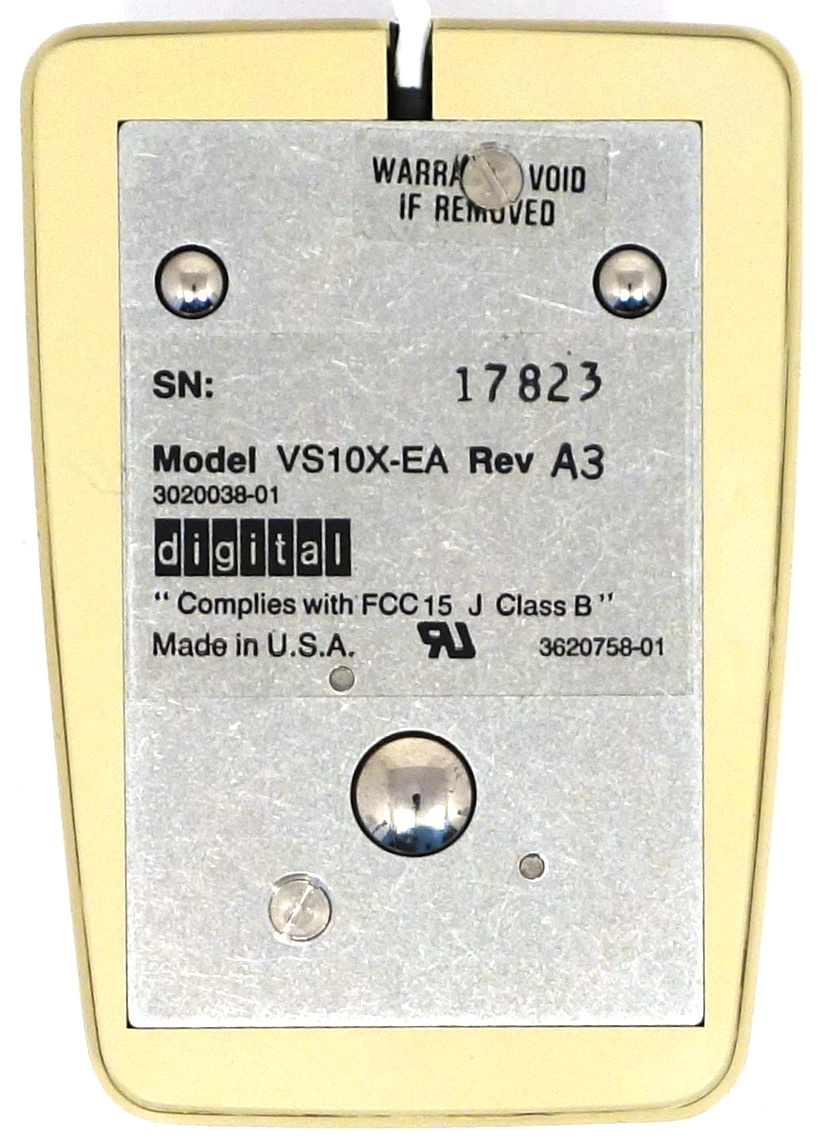
\includegraphics[scale=0.5]{1983_dec_vs10x_ea_mouse/bottom_30.jpg}
    \caption{DEC VS10X-EA Mouse, вид сверху и снизу}
    \label{fig:DecVS10XTopAndBottom}
\end{figure}

Нижняя сторона целиком выполнена из металла (рис. \ref{fig:DecVS10XTopAndBottom}). Вращение регистрируется гладким стальным шаром в центре, а еще два шарика меньшего размера играют роль ножек для минимизации трения. Мышь не комплектовалась ковриком: руководство пользователя VAXstation 100 предлагает использовать в этом качестве обычный лист бумаги \cite{manual}.
 Съемное кольцо, позволяющее извлечь шар для удаления собравшегося мусора, в данной модели еще не предусмотрено, поэтому для чистки необходима полная разборка.

\begin{figure}[h]
    \centering
    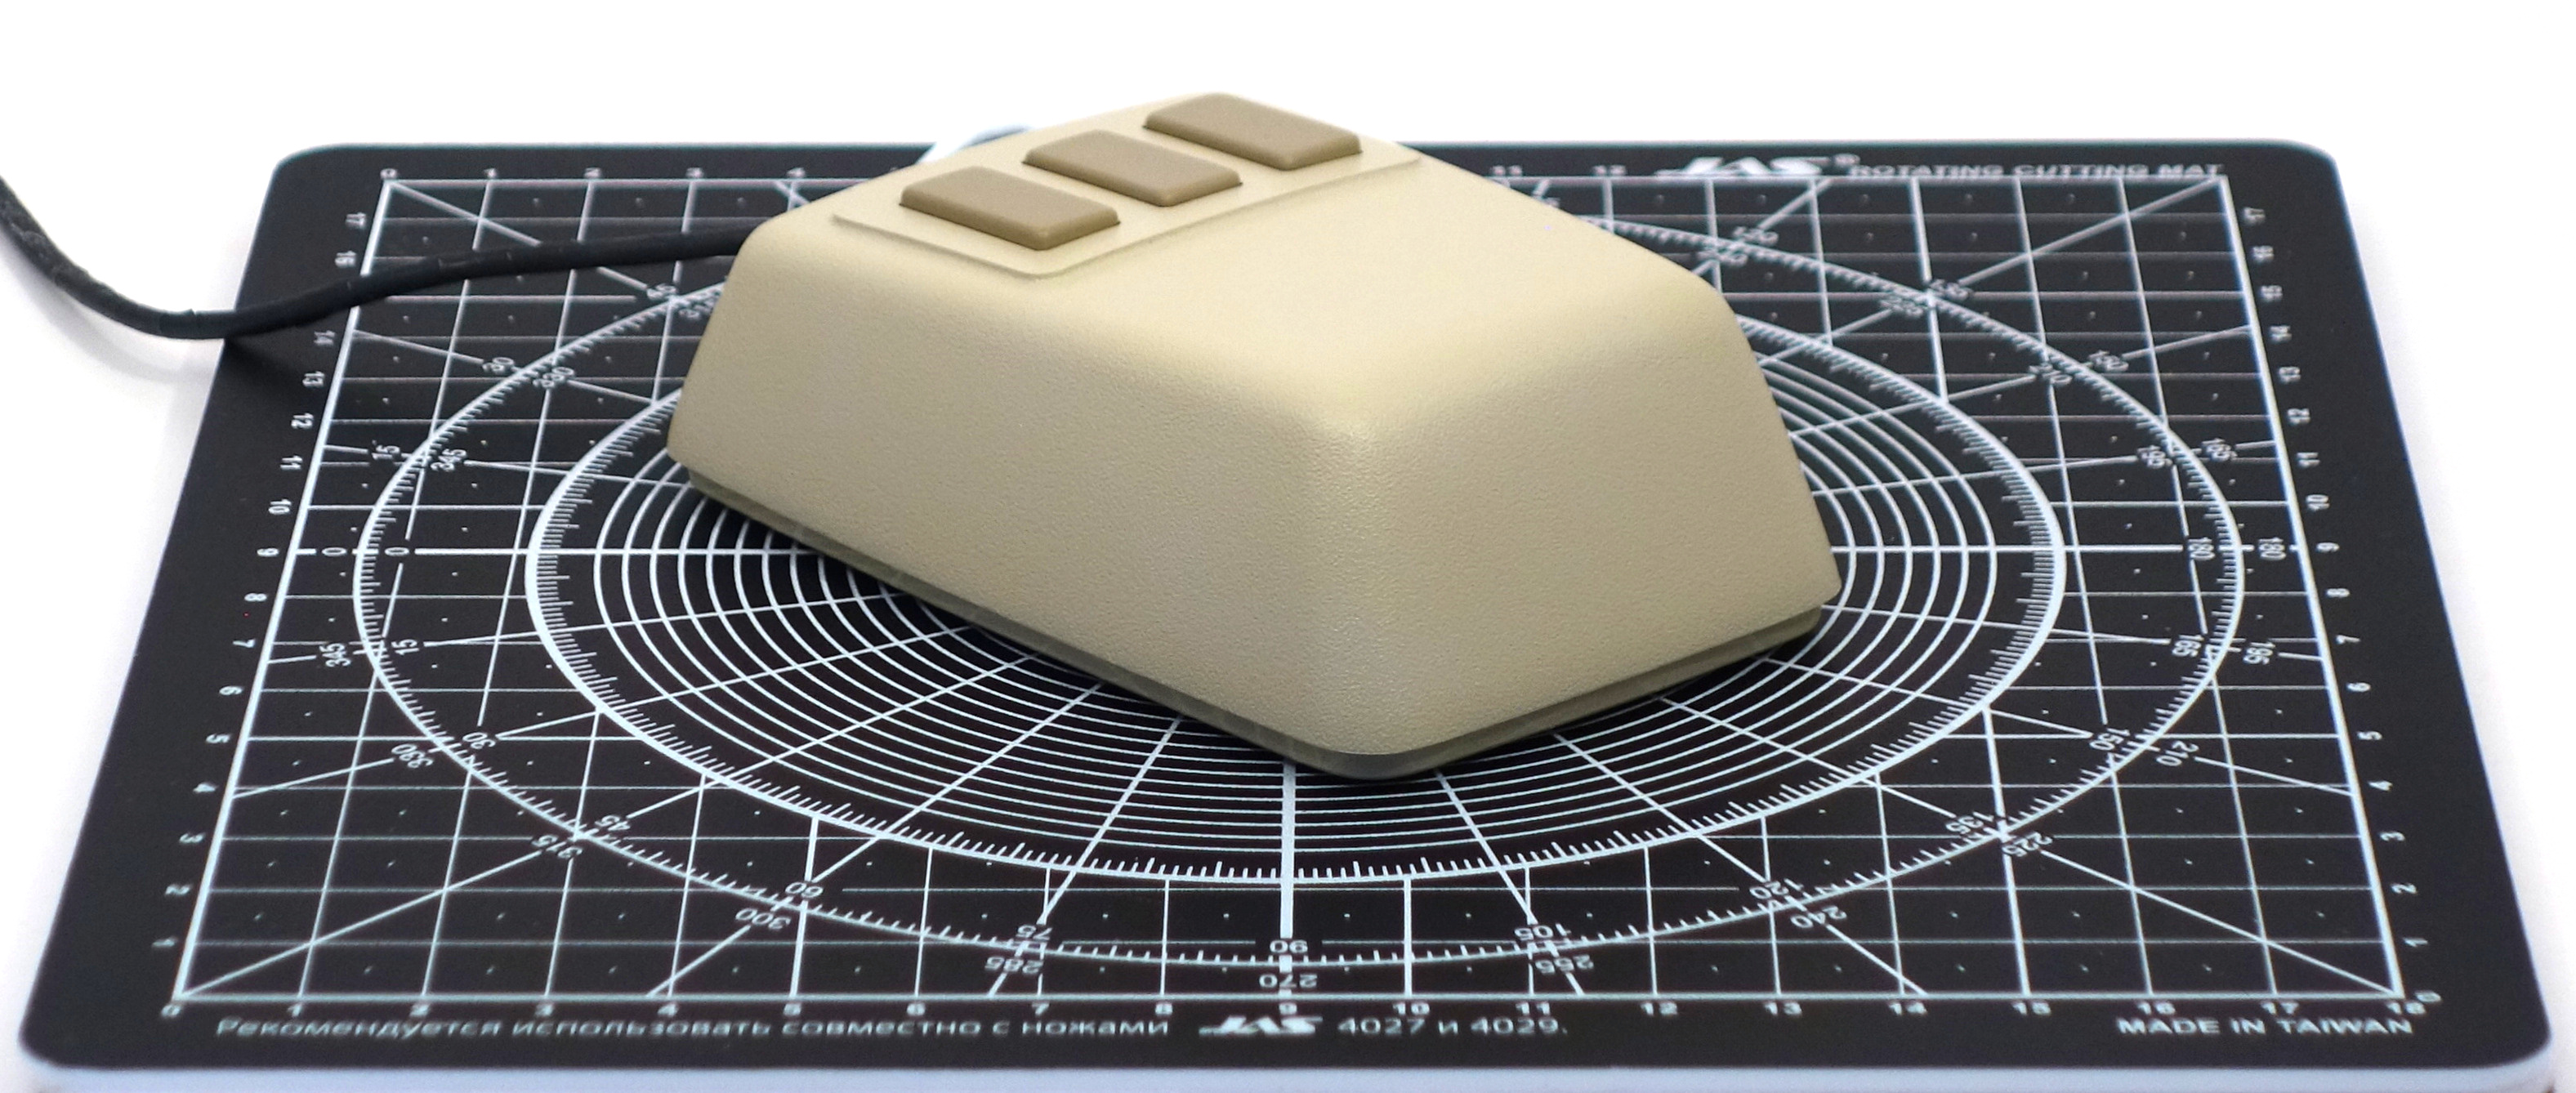
\includegraphics[scale=0.7]{1983_dec_vs10x_ea_mouse/size_30.jpg}
    \caption{DEC VS10X-EA на размерном коврике с шагом сетки 1~см}
    \label{fig:DecVS10XSize}
\end{figure}

Мышь имеет небольшие размеры, характерные для мышей 1980-х годов (рис. \ref{fig:DecVS10XSize}); рука опирается на корпус лишь в незначительной степени (рис. \ref{fig:DecVS10XHand}).

\begin{figure}[h]
    \centering
    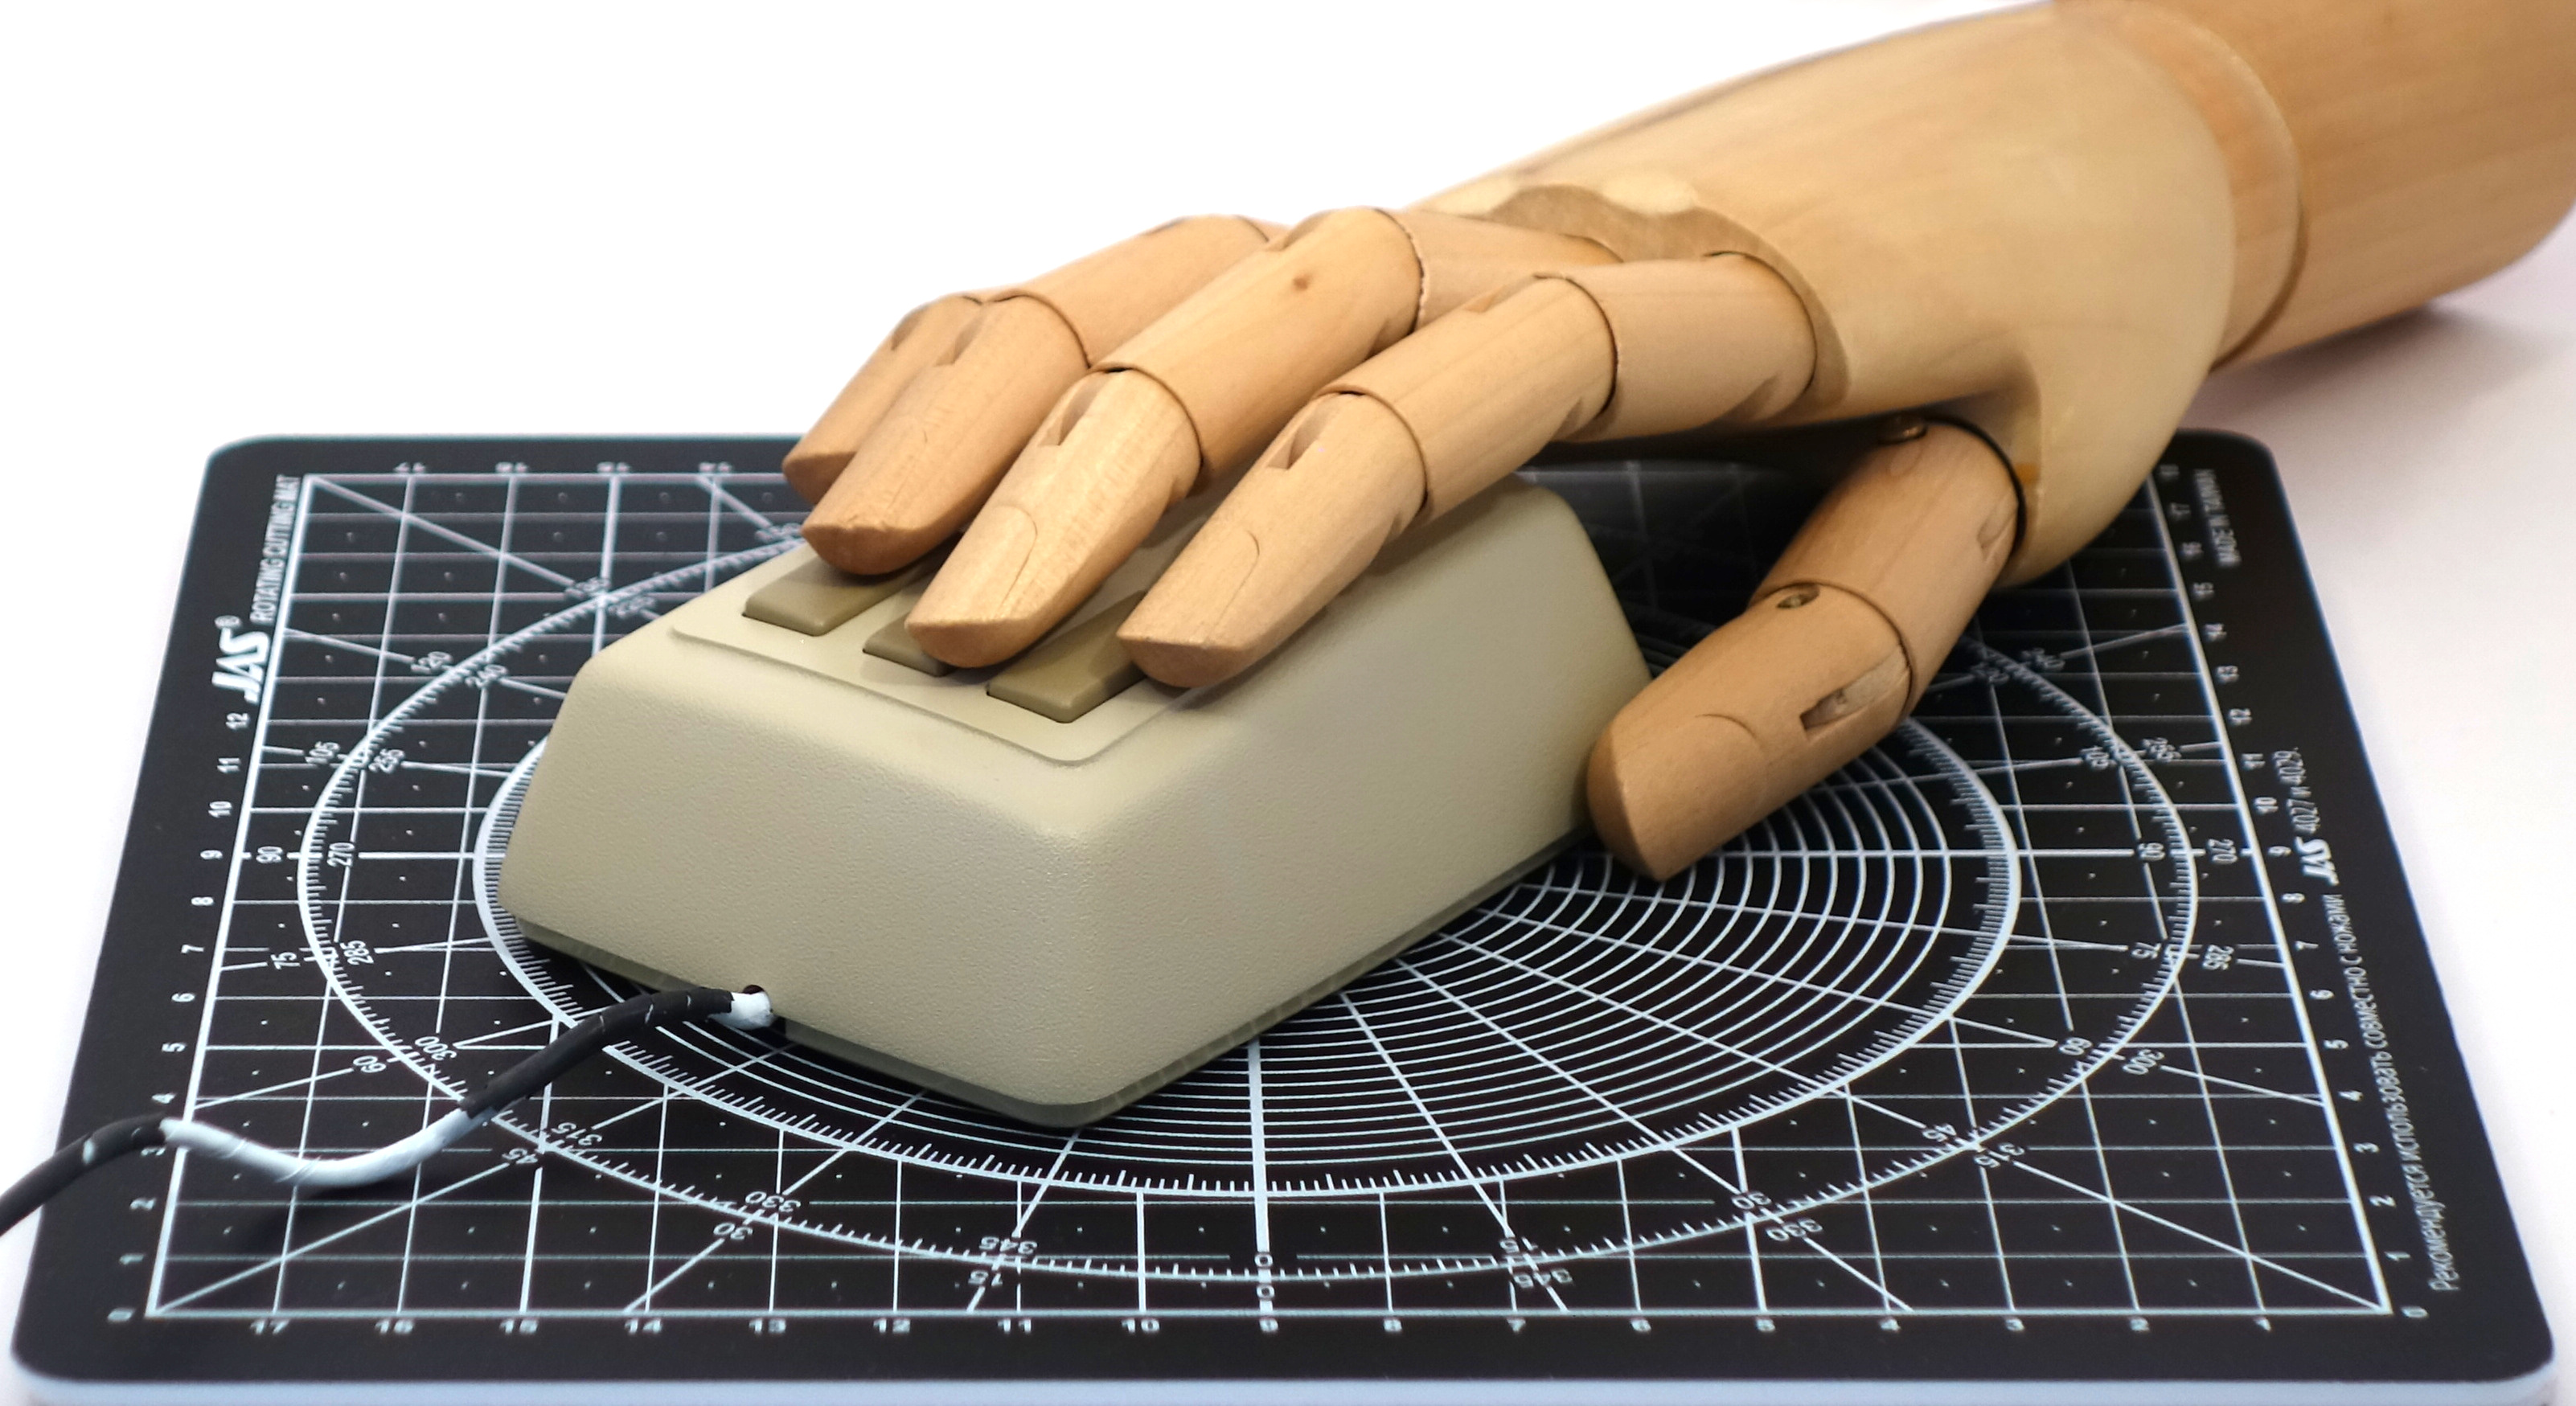
\includegraphics[scale=0.7]{1983_dec_vs10x_ea_mouse/hand_30.jpg}
    \caption{DEC VS10X-EA с моделью руки человека}
    \label{fig:DecVS10XHand}
\end{figure}

Внутреннее устройство мыши показано на рис. \ref{fig:DecVS10XInside}. Можно отметить съемную глухую защиту шара, требующую дополнительных операций разборки для удаления мусора. В мыши использованы контактные энкодеры (с четырьмя контактами для большей надежности), включающие в себя металлический контактный барабан, вместо более распространенного в последующих моделях диска.

 \begin{figure}[h]
    \centering
    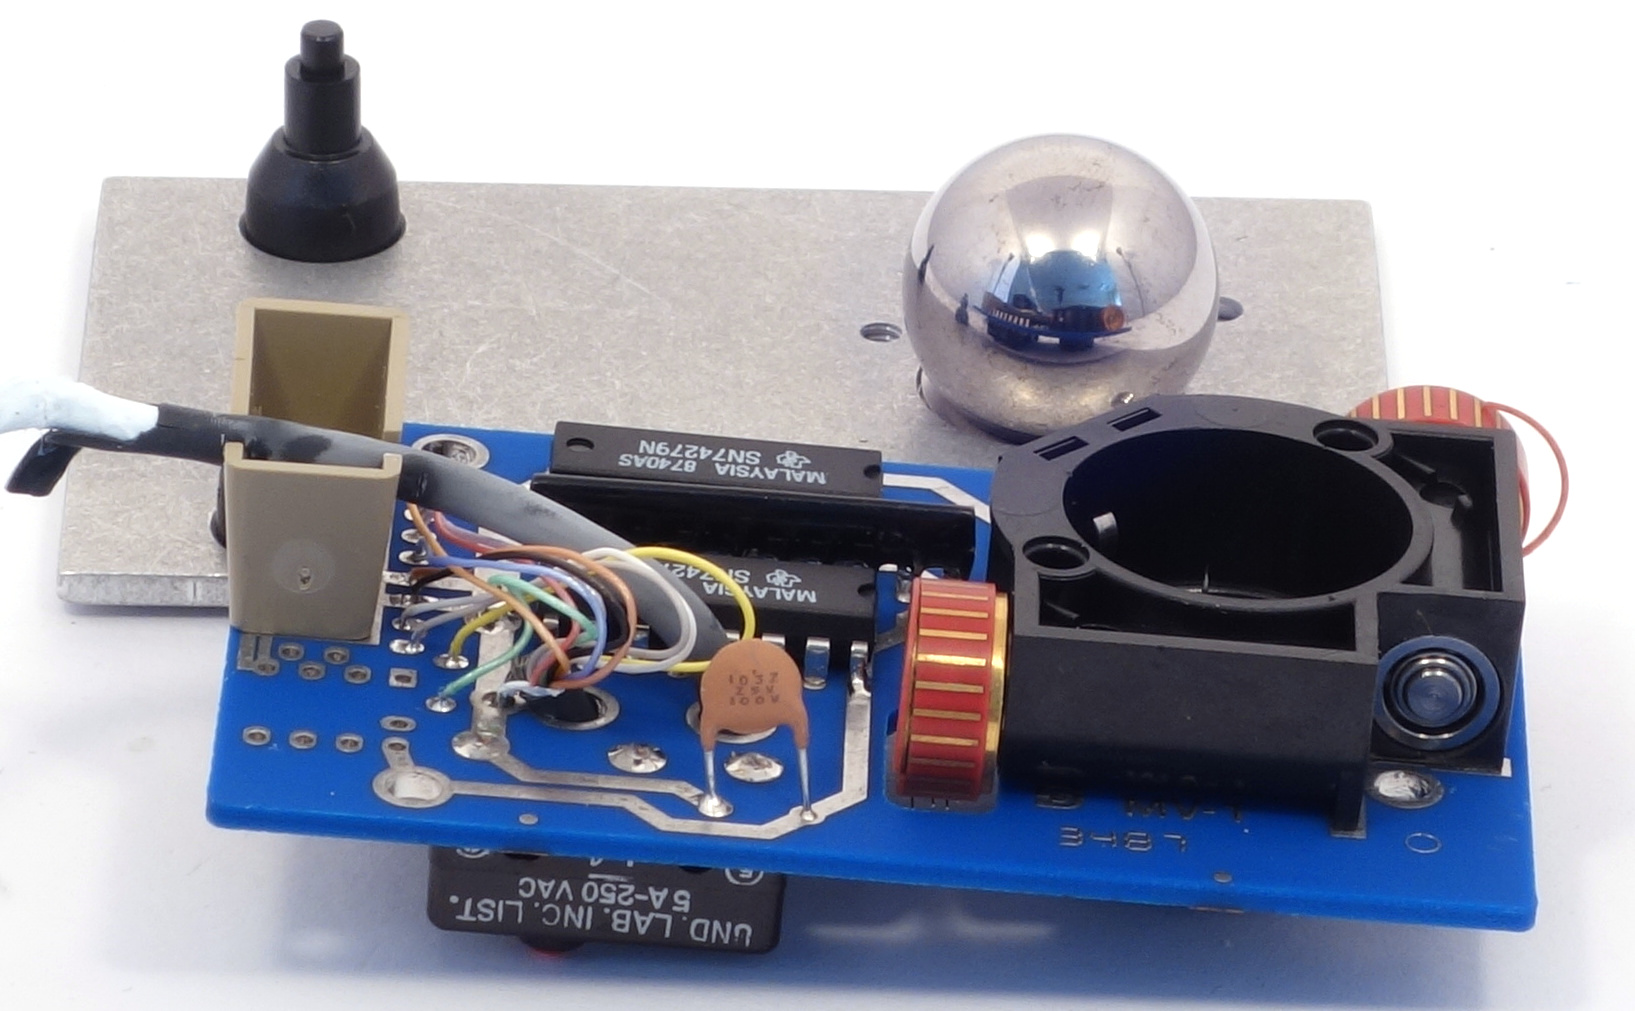
\includegraphics[scale=1]{1983_dec_vs10x_ea_mouse/inside_30.jpg}
    \caption{DEC VS10X-EA в разобранном виде}
    \label{fig:DecVS10XInside}
\end{figure}

\begin{thebibliography}{9}
\bibitem{hawley} Hawley Mouse House \url{https://oldmouse.com/mouse/hawley/}

\bibitem{mouses} Hawley Mark II X063X Mouses \url{https://oldmouse.com/mouse/hawley/X063X.shtml}

\bibitem{pat} Transducer for a display-oriented pointing device \url{https://patents.google.com/patent/US3892963A/en}

\bibitem{reddit} Another DEC mouse \url{https://www.reddit.com/r/vintagecomputing/comments/mm4des/another_dec_mouse/}

\bibitem{manual} VAXstation 100 User Guide \url{http://www.bitsavers.org/pdf/dec/vax/vaxstation100/AA-N660A-TE_VAXstation_100_Users_Guide_Jun84.pdf}
\end{thebibliography}
\end{document}
